% !TEX TS-program = pdflatex
% !TEX encoding = UTF-8 Unicode

\chapter{State of the Art} \label{chapter:sota}

	%\pagenumbering{arabic}


\section{Genome Sequencing}

Over the last years of genome sequencing innovation, a shift has been seen from the more traditional Automated Sanger sequencing to cheaper and faster Next Generation Sequencing techniques. For a quick overview, the Sanger method starts of with either bacterial cloning or a Polymerase Chain Reaction to amplify the \gls{DNA} strands. It is followed by four reactions containing deoxynucleotides and \gls{DNA} Polymerase performed separately for each to include a different dideoxynucleotide (ddNTP). When a ddNTP that binds to a specific deoxynucleotide is attached to an elongating \gls{DNA} chain, the \gls{DNA} polymerase stops it's process on it, thus labelling every nucleotide. The ddNTPs are radioactively or fluorescently marked so that the final sequence can be visualized on the gel electrophoresis image, such as in the figure \ref{sanger} \cite{sanger1977dna}.

\begin{figure}
	\centering
	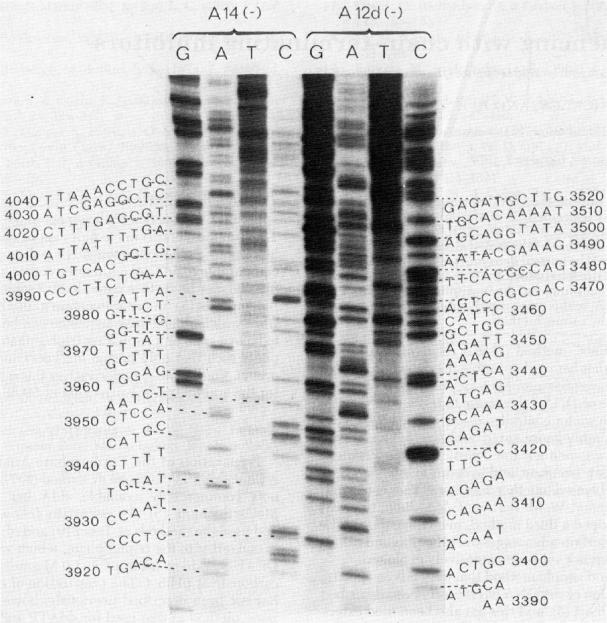
\includegraphics[width=3.628in]{../images/data_prep/sanger1977dna.jpg}
	\caption{Picture of the acrylamide gel electrophoresis with the sequences read annotated on the sides. From left to right, the inhibitors used are ddGTP, ddATP, ddTTP, and araCTP. Adapted from "DNA sequencing with chain-terminating inhibitors" \cite{sanger1977dna}.} 
	\label{sanger}
\end{figure}

The most recent implementations of this method can achieve extremely high genotyping accuracies, but are expensive, time consuming, and better suited for only single gene sequencing. Since there was a need for cheaper processes with larger throughput capabilities, Next Generation Sequencing emerged. The single major advantage provided by this new technology it's is ability to output enormous amounts of data in a single run, cheaply and fast. \gls{NGS} methods start off by randomly fragmenting the \gls{DNA}, and coupling adapters to both ends of the fragments. These are then attached to a flow cell and amplified in clusters that are recorded by various pictures. This produces a great number of short reads that are then anchored to a reference genome, where small differences can be determined. The number of base pairs contained in every read, and the number of reads depend on the sequencer itself \cite{ansorge2009next}. Further description and visualization of this process can be found in the figure \ref{ngs-sequencing}.

Generally, genome studies only target the exome because it contains the protein coding regions \cite{choi2009genetic}. However, it has also been shown that many variants that are associated with disease can be found on non coding regions of the genome \cite{manolio2009finding}. For this reason, it became increasingly important to integrate \gls{WGS} techniques when performing \gls{GWAS}. Nonetheless, the cases data utilized in this study are only of the exome. 

From the data recovered, it is then possible by using reference panels of known \gls{SNP}s or other variants to produce \gls{VCF} files, that record the genotype for each variant \cite{zook2014integrating,mccarthy2016reference}. There are several programs available to perform variant calling from the short reads aligned to a reference genome, such as SAMtools $(http://samtools.sourceforge.net/)$. These can do this process in many different ways, but the main goal is to identify where the reads differ from the reference genome and to translate those to a \gls{VCF} file.

%\newpage

\begin{figure}
	\centering
	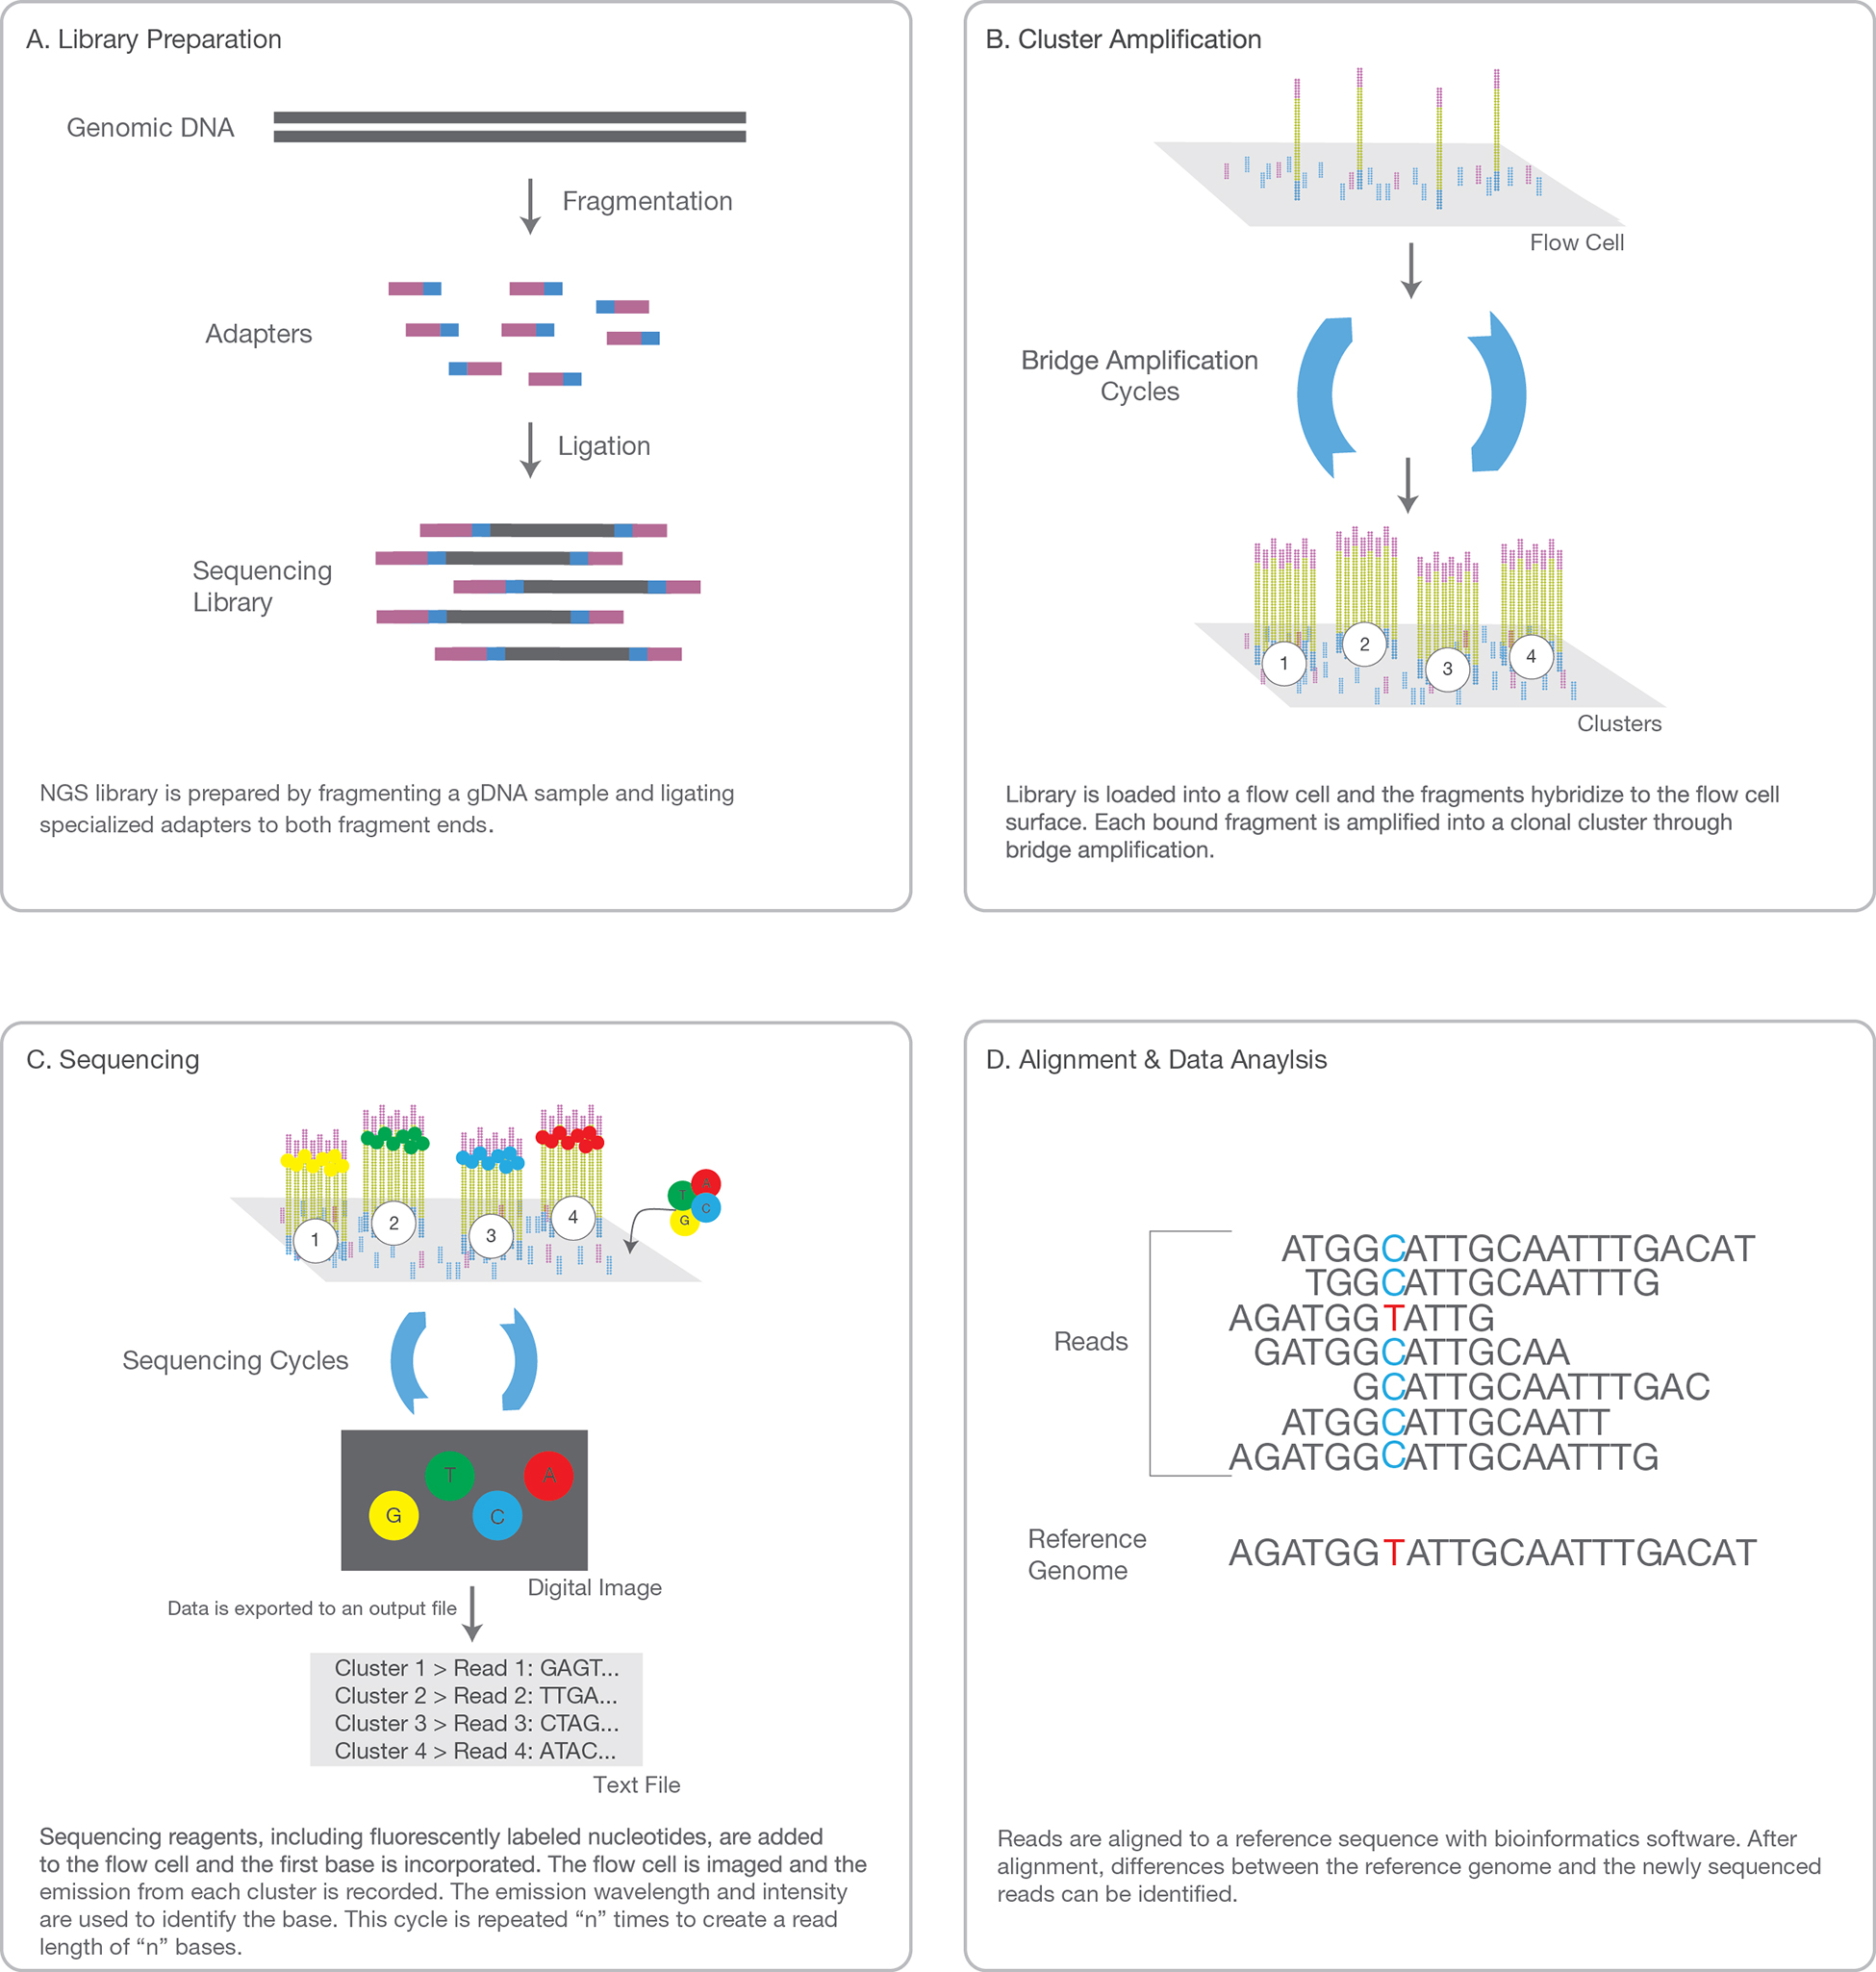
\includegraphics[width=\textwidth]{../images/data_prep/ngs-sequencing-workflow.jpg}
	\caption{Work flow of the Next Generation Sequencing Techniques employed by Illumina sequencers. Adapted from Illumina's images for general use.} 
	\label{ngs-sequencing}
\end{figure}

\newpage

\section{Variant Call Format}

Nowadays, as previously stated, information of the genotypes assembled from the sequencers are represented in a Variant Call Format files, or \gls{VCF} files. These start with the meta information lines, which indicate the \gls{VCF} version, followed by the three possible parameters INFO, FILTER and FORMAT. INFO describes any additional information of the metrics collected for every variant and FILTER describes what kind of filters were applied to them. FORMAT indicates the type of genotyping information that is present and it's characteristics. Then, the header line ensues which presents the following 8 fixed columns: \#CHROM, POS, ID, REF, ALT, QUAL, FILTER, INFO. These represent respectively the chromosome of the variant, it's position in it, a sample ID, the bases for the reference genome, the bases for the possible alternative bases for the variant, the quality or certainty of the genotype, any filters applied that were previously described and any additional info for the variant. If there is genotype information present, then a FORMAT columns ensues, which dictates how the genotypes are going to be presented, followed by the actual genotypes for a set number of samples. All the following lines represent existing variants that were genotyped. More information on this file type can be found at $https://github.com/samtools/hts-specs$ .

\section{Single Marker and Multi-locus Analysis and Imputation}

%After the first mapping of the human genome, on May 27, 2004, the costs of sequencing started to go down, while the number of genome projects published rose \cite{schmutz2004quality}. 
%As such, while large and numerous datasets became available, scientists started to develop new ways to analyse and research them. 

Since 2007, \gls{GWAS} have been responsible for the discovery of genetic markers that relate to complex human traits and disorders, the simplest approach being the Single Marker Analysis, which is both capable of finding common variants with addictive effects and rare ones with high phenotype impact \cite{scott2007genome}.
 
This marker-by-marker analysis focus on the individual effect of each variant, to detect associations between molecular markers and traits or disorders in a population. These close groups of variants that are discovered to be correlated to a certain phenotype are called Quantitative Trait Loci. In many complex diseases, several \gls{QTL}s are discovered because of Linkage Disequilibrium, that refers to the non-random association of alleles at different loci in a population, and it's visible when their association frequency is higher or lower than what would be expected if it was in fact random \cite{slatkin2008linkage}. It is influenced by many factors, such as rate of mutation, population structure, genetic linkage, the rate of mutation, genetic drift and the system of mating, and can signal segments in the chromosomes that trace back to a common ancestor without intervening recombination. Essentially, the objective is to determine if phenotype differences are due to a few loci with large effects or many loci with small, but additive ones.  

We can formalize a contingency table that contains the information of the genotype for each \gls{SNP}, and the corresponding phenotype for each sample, and use tests such as \textbf{Pearson's $\chi^2$ Test}, \textbf{Fisher's Test} and \textbf{G-Test} to detect an association between allele frequencies and phenotype \cite{zhang2012mining}. Since the \textbf{Pearson's $\chi^2$ Test} is going to be used, a short description follows. Normally, this test is used to verify if there is a deviance of the expect frequencies and the observed frequencies. It's null hypothesis is that the data are independent, and by rejecting this hypothesis, we can then find associations between them. This test assumes the data follows a normal distribution, and it's given by \cite{pearson1900x}: 
\begin{equation}
	\chi^2 = \sum_{i = 1}^{k}\frac{(x_i - m_i)^2}{m_i} \\
\end{equation}
 
To go even further and detect a \gls{QTL} with this approach, the association between a marker and a trait, or in this particular case, Type 2 Diabetes, can be modelled by simple regression methods \cite{haley1992simple}. The null hypothesis for these tests is that the marker has no association with the trait, and to test it, a t-test, F-test or Bayes factor can be used. We assume that a marker will only affect the desired trait if it is in \gls{LD} with a \gls{QTL}. To measure \gls{LD}, considering A and B as two different markers, A1, A2, and B1, B2 as their alleles respectively:
\begin{equation}
D = frequency(A_1\_B_1)\times frequency(A_2\_B_2) - frequency(A_1\_B_2)\times frequency(A_2\_B_1) \\
\end{equation}

, $frequency(A_1\_B_1)$ being the frequency of the haplotype $A_1\_B_1$, and likewise for the remaining haplotypes. Since this is very dependant on allele frequencies, the $r^2$ metric was proposed:
\begin{equation}
r^2 = \frac{D^2}{frequency(A_1)\times frequency(A_2)\times frequency(B_1)\times frequency(B_2)}\\
\end{equation}

By combining $r^2$, LD and the number of markers in the study we can infer the power of the association test to detect \gls{QTL}s \cite{hill1968linkage,visscher201710}. 

The following approach tried was the Multi-Locus analysis. It was the next logical step, because it tries to tackle issues that were not handled in the previous methods, such as epistasis and big marker spacing (less genotyped variants) \cite{mooney2012ga}. It is fairly recent, and its objective is to consider various locus and their interactions when performing the association studies. When building marker-to-marker association models, if our set contains 1 million \gls{SNP}s, it becomes both statistically and computationally hard to differentiate between significant markers and to understand their biological context, as there will be $5\times10^{11}$ interactions to examine \cite{turner2011knowledge}. Although a Multi-Locus analysis adds several benefits to it's previous iteration, it requires even more processing power. At this point, feature selection comes into play, there being several ways to approach it. The most common ones are the usage of \gls{SNP}s that have met certain criteria in broader previous tests or integrating biological knowledge in the models. Of course, either one of these strategies imposes bias, such as eliminating potential markers that don't prove to have a significant effect on their own, and missing novel undocumented interactions \cite{carlson2004mapping}. By considering a smaller number of \gls{SNP}s in which the phenotype information might be contained, it becomes possible to make such an analysis. One example of this approach is the Biofilter, that uses previous Biological knowledge to construct several multi-SNP models, and only then applies Logistic Regression and Multi-factor Dimensionality Reduction methods to perform its analysis \cite{bush2012genome,bush2009biofilter}.

To increase the number of \gls{SNP}s available and generate a common set of genotyped variants for each dataset, for Genome Wide Association Studies, Imputation surfaced as a viable candidate. By using known Linkage Disequilibrium patterns and frequencies of haplotypes from the 1000 Genomes Project, it is possible to make a correct estimate of missing genotypes. However, imputation leads to the underlying assumption that the study population has the same patterns of \gls{LD} and that the association between haplotypes and causal loci is the same in the reference population, which might not always be the case \cite{10002012integrated, bush2012genome}.

\section{\textit{Bayesian} Methods}

The usage of previously explained \textit{frequentist} methods, although very widely used, still pose some problems because of a limitation on the usage of \textit{p-values} themselves. From a \textit{p-value} alone it is very hard to know how confident it is possible to be when a \gls{SNP} is associated with a phenotype \cite{ioannidis2008effect}. Furthermore, the datasets used in these studies are usually small, an it is necessary to account for their uncertainty \cite{o2008bayesian}. By using \textit{Bayesian} methods we can circumvent these issues, at the expense of additional assumptions about the influence on phenotype for each \gls{SNP}. Another great advantage of these methods is that they allow for a common-ground when comparing results between studies (\textit{meta-analysis}), facilitating knowledge integration \cite{stephens2009bayesian}. It turns the probability that a \gls{SNP} affects a phenotype in a quantitative measure, the Bayes Factor:
\begin{equation}
	BF = \frac{P(data | \theta_{het} = t_1, \theta_{hom} = t_2)}{P(data | \theta_{het} = 0, \theta_{hom} = 0)}
\end{equation}

For these reasons, \textit{Bayesian} methods have become more prevalent in recent years in GWAS \cite{fernando2017application}. It is also readily usable in several packages, such as SNPTEST \cite{marchini2007new}, genMOSS \cite{friedlander2016analyzing} and BIMBAM \cite{guan2008practical}.

\section{Dimensionality Reduction}

However, even with such techniques, the missing heritability is still yet uncovered for complex diseases, which leads us to Epistasis or gene-gene interaction, and how to integrate it in \gls{GWAS}. These are some of the methods available that can enable Multi Locus analysis. When accounting for gene-gene interactions, as stated before, the problem becomes statistically and computationally complex, since for the three possible genotypes and $k$ \gls{SNP}s, there are $3^k$ genotype classes possible \cite{winham2013applications}. To attenuate these issues, and combine variants information considering gene-gene interaction, Dimensionality Reduction can be used. Usually these problems entertain very large numbers of \gls{SNP}s so combining their information in a smaller number of vectors while still retaining most of their variance information can make it extremely easier to analyse these kinds of datasets. There are several methods that can perform this reduction, such as \gls{MDR}, \gls{PCA} and \gls{LDA}.

 At it's core, \gls{MDR} is an algorithm capable of constructing new features by pooling genotypes from multiple \gls{SNP}s \cite{moore2006flexible}. Considering several multi locus genotype information and given a threshold T, a certain group of \gls{SNP}s is considered high risk if their ratio of case study to control group is higher than T, or low risk if that same ratio is lower \cite{moore2010bioinformatics}. By doing so, a new one dimension vector with two different groups (High and Low risk) is constructed, which enables the usage of other techniques to process it, and produce multi locus analysis results. 

The \gls{PCA}'s goals are to extract a set of new orthogonal variables of a dataset, called the Principal Components, that are able to represent the important information in a k number of vectors \cite{abraham2014fast}. To do so, a p-dimensional vector of weights $W_{(k)} = (w_1, w2, ..., w_p)_{(k)} $ that map to each row of our dataset matrix X will be worked out. To calculate the first component we maximize the variance: 
\begin{equation}
W_{(1)} = arg\  max \Big\{ \frac{W^T X^T XW}{W^T W} \Big\} 
\end{equation}
, which is the largest eigenvalue of X when W is the corresponding eigenvector. The first Principal Component will then be given by $t_{1i} = X_{(i)} \cdot W_{(1)}$ \cite{bro2014principal}. Considering $n$ observations and $p$ features, this method can output several $\min{n-1, p}$ vectors containing the highest variance of the data possible. This method is usually used in \gls{GWAS} to detect population structure and outliers \cite{price2006principal}.

The last dimensionality reduction method covered is Linear Discriminant Analysis and it makes use of the data labels to propose a linear combination of variables that best maximize the classes separation. It is then, contrary to \gls{PCA}, called a supervised algorithm. Regarding a binary problem, which happens to be most of phenotypic studies, for each class in $y$, mean and covariance are represented by $\mu_0$ / $\sum_0$ and $\mu_1$ / $\sum_1$ respectively. A function of the linear combination of samples can be obtained by:
\begin{equation}
\overrightarrow{w} \cdot \overrightarrow{x} > c
\end{equation} 
where, 
\begin{equation}
\overrightarrow{w} = \sum ^{-1}(\overrightarrow{\mu_1} - \overrightarrow{\mu_0})
\end{equation}
\begin{equation}
c = \frac{1}{2} (T - \overrightarrow{\mu_0}^T\sum_{0}^{-1} \overrightarrow{\mu}_0 + \overrightarrow{\mu_1}^T\sum_1^{-1}\overrightarrow{\mu_1})
\end{equation}
and $T$ is a threshold that verifies the following condition:
\begin{equation}
(\overrightarrow{x} - \overrightarrow{\mu_0})^T \sum_{0}^{-1}(\overrightarrow{x} - \overrightarrow{\mu_0}) + \ln \abs{\sum_0} - (\overrightarrow{x} - \overrightarrow{\mu_1})^T \sum_{1}^{-1}(\overrightarrow{x} - \overrightarrow{\mu_1}) - \ln \abs{\sum_1} > T
\end{equation}
The new hyperplane defined by $c$, is then the one that maximizes the separability of classes. It can be used either for classification or to reduce dimensionality of a dataset \cite{izenman2013linear}.

These approaches have been widely and successfully used in other \gls{GWAS} studies, and improved with entropy-based interpretation methods, the use of odds ratio, imputation, parallel implementations and much more \cite{moore2006flexible}. Furthermore, cases like the susceptibility to bladder cancer were found in highly significant interactions between \gls{SNP}s using such methods that consider epistasis, with higher prediction power than smoking \cite{stern2009polymorphisms}. 


\section{Quality Control and Validation}

When performing a \gls{GWAS}, the ultimate goal is for it to be able to predict, in any new given dataset, the interaction of markers and phenotypes that were discovered. To be able to validate this work, it is extremely important to test the results in data sets that were not used during the study, since most significant effects uncovered are likely to be overestimations \cite{xu2003theoretical}. In \gls{GWAS}, there are far more \gls{SNP}s than number of samples, which can easily lead to a model that predicts all cases in the discovery dataset and that cannot be replicated in others. This is called over-fitting \cite{hayes2001prediction}. Furthermore, validation leads to a higher confidence level in the study performed, and also allows to uncover the populations where it can be replicated, if at all. Validation must be first thought out when designing the study, by assigning a percentage of samples to perform testing and other for cross-validation (apart from training).

As most of the studies samples are from a single population, the choice of control group must also take that into consideration as a risk variant might not be relevant across all different populations. Most control groups can be gathered from the study itself, but to promote less bias, samples from the 1000 Genome Project can be used \cite{10002012integrated}. This project gathered variants from populations across the world, that serve not only as control, but as gold standards for imputation.

The verify the quality of the genotypes themselves, it is possible to use the Hardy-Weinberg Equilibrium \cite{hosking2004detection}. The \gls{HWE} is a model that states genotype frequencies follow certain rules, and remain constant at each generation \cite{wigginton2005note}. Some factors that can affect this equilibrium include migration, mutation, natural selection and assortative mating (tendency for people to choose partners who are more phenotypically similar or dissimilar to themselves). However, if these factors are negligible in the target population, deviations from the \gls{HWE} are most likely due to incorrect genotyping. Considering $f(A) = p$ and $f(a) = q$, the expected genotypes frequencies are then:
\begin{equation}
	f(AA) = p^2
\end{equation}
\begin{equation}
f(aa) = q^2
\end{equation}
\begin{equation}
f(Aa) = 2pq
\end{equation}
As such, the \gls{HWE} should follow the curved line in the De Finetti diagram displayed in figure \ref{fig:HWE}.

\begin{figure}[h]
	\centering
	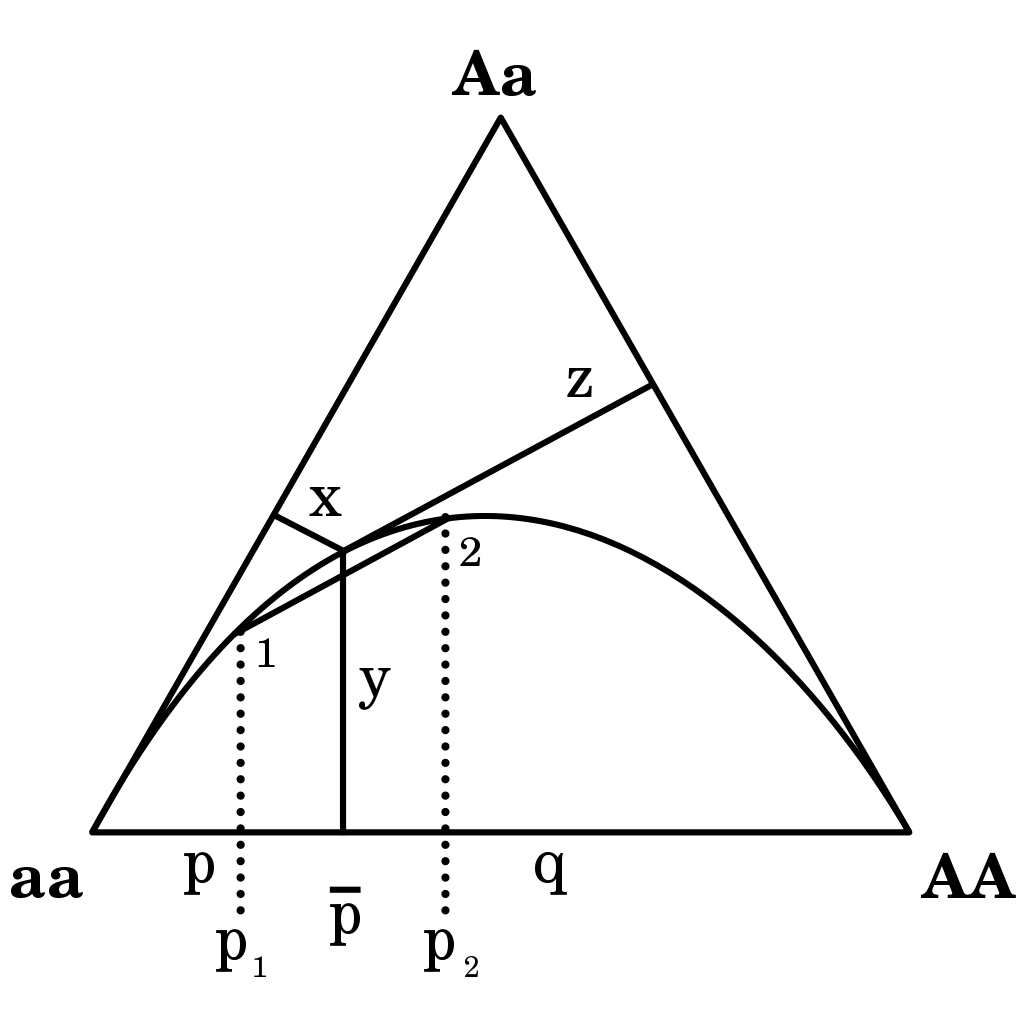
\includegraphics[width=3in]{../images/sota/1024px-De_Finetti_diagram.png}
	\caption{De Finneti diagram of genotype frequencies. If a population follows the Hardy-Weinberg Equilibrium, their genotype frequencies distribution will follow the curved line on the plot. Free licensed image from Wikimedia Commons.} 
	\label{fig:HWE}
\end{figure}


\section{Data Mining and Machine Learning}

In genomics, the vast quantities of data that must be scouted before any meaningful results are achieved is daunting, and simple frequentist methods have not yet been able to fully crack the problem of complex diseases heritability. As we inquire further the study of gene-gene or gene-environment interactions and non-linearity in the mapping of genotype to phenotype to understand genomic variation, disease susceptibility and the role of environment in genomics, it is important to evaluate how these situations are approached. There might be a combination of \gls{SNP}s that, if addressed with the proper non-linear function, can significantly translate into the respective phenotypes, but each \gls{SNP} individual contribution might not appear any different than the millions of other \gls{SNP}s. To this outcome, that can't be predicted by the sum of all markers, it is called non-linearity \cite{moore2010bioinformatics}.

To produce non-linear models, it first must be discussed how to effectively reduce the amount of SNPs that a model needs to look through, or in other words, how to data mine the genome. At this point, the scientific community is slowly transitioning to non-linear analysis of the genome, but there aren't many methods developed so far \cite{marjoram2014post}. A model can also be built without any preprocessing, but besides the great quantity of features for few samples, a great majority of the millions of SNPs available are considered either noise or non-significant to the task at hands. There are essentially 2 types of feature selection used, which are the filtering and the wrapper approaches \cite{moore2010bioinformatics}. The first one, refers to the preprocessing of data and assessment of the quality and significance for each feature, to ultimately collect a significant subset. The wrapper one utilizes a deterministic or stochastic algorithm that iteratively selects subsets of data to classify. Filtering is a faster approach, while the wrapper can be more powerful, since it doesn't discard variables with assumptions of quality. Even if these two methods are widely used, there are multiple other ways of discarding noisy \gls{SNP}s, for example, the inclusion of biological knowledge \cite{xu2009snpinfo}. 

After the preprocessing methods are carefully selected and implemented, and subsetting has been performed, machine learning can be used to classify between the desired phenotypes. The purpose of machine learning is to make computers learn how to perform certain tasks, by providing them with a set of examples, but without explicitly programming them to do so. In our problem context, each variant is considered a feature, which means that it is an attribute from where the model can learn. The entirety of features and samples compose the training dataset. To provide the machine with the context of what to learn, a target vector is given. This vector contains information on the phenotype that requires classification \cite{nelson2013higher}. The most popular machine learning methods are Support Vector Machines, Decision Trees, Naïve Bayes classifiers, Neural Networks and Fuzzy Sets \cite{szymczak2009machine}. Since there is a growing interest in non-linear models, \gls{SVM}s, Decision and Neural Networks are some of the most promising Machine Learning Methods \cite{kavakiotis2017machine}. On this project, \gls{SVM}s and Decision Trees were used, so a more complete description is provided for them.

For explanation purposes, let's consider the binary classification problem, with linearly separable classes and only two features for the \gls{SVM}. A Support Vector Machine tries to ensure the largest possible boundary between both classes. To do this, it produces two support vectors to the main decision boundary, that provide the largest distance possible between the closest instances from each class \cite{hearst1998support}. This process can be better understood through figure \ref{fig:svm_func}. When more features are added to the problem, it stops being viewable in plots, since the dimensionality of the problem grows, but the same principle is applied.

\begin{figure}[h]
	\centering
	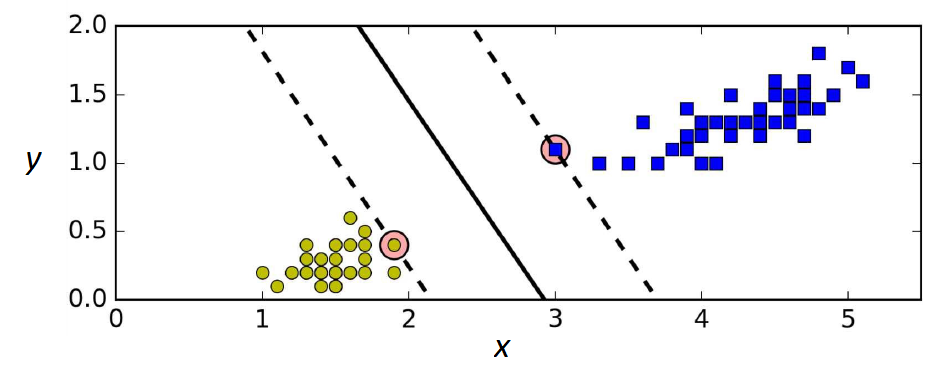
\includegraphics[width=\textwidth]{../images/results/svm_func.png}
	\caption{Plot of two classes separated by the support vectors on the dashed lines, and the decision boundary on the black line at the centre. Adapted from the book "Hands on Machine Learning with Scikit-Learn and TensorFlow" \cite{geron2017hands}.} 
	\label{fig:svm_func}
\end{figure}

However, this mechanism assumes that there are no instances overlapping which is something very likely to occur in a "real-life" dataset. To then handle it, a soft margin classification can be implemented. What it does, is allow for some violations of the margins that support vectors provide, which makes for a wider distance between them. By doing this, it is also much more likely that the classifier will generalize better. The parameter that handles the number of violations allowed is C \cite{geron2017hands}. The higher it is, the fewer the violations and consequent distance of support vectors. An example of $ C = 1 $ can be seen in figure \ref{fig:linear_svm}.

\begin{figure}[h]
	\centering
	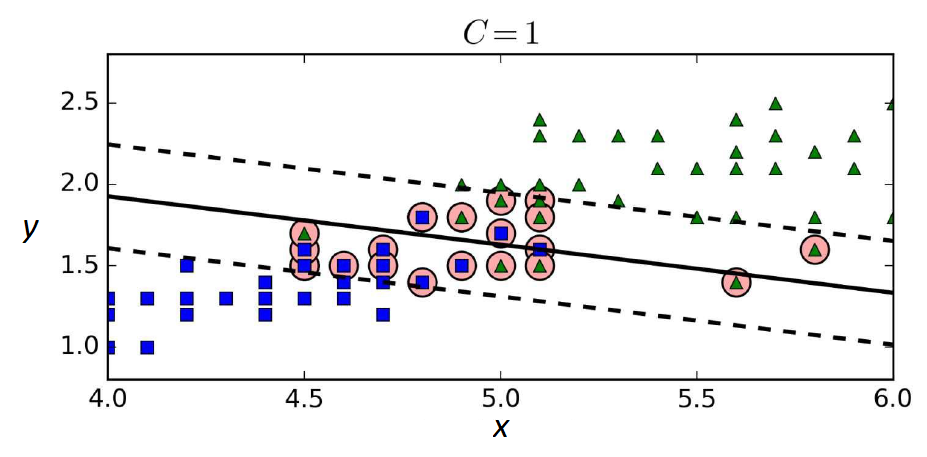
\includegraphics[width=\textwidth]{../images/results/linear_svm.png}
	\caption{Plot of \gls{SVM} adjusting to two features with $C=1$. Adapted from the book "Hands on Machine Learning with Scikit-Learn and TensorFlow" \cite{geron2017hands}.} 
	\label{fig:linear_svm}
\end{figure}

Although this classifier is very powerful, a very large number of datasets cannot be linearly separable. To solve this, extra features that are transformations of the original ones are added, that allows for a different arrangement of data. An example of this process can be seen in figure \ref{fig:svm}. However, performing such great number of transformations can turn extremely computationally heavy which lead to the implementation of the \textit{Kernel Trick}. This trick is intended to calculate the dot product of the transformed vectors without having to transform them \cite{geron2017hands}.

\begin{figure}[h]
	\centering
	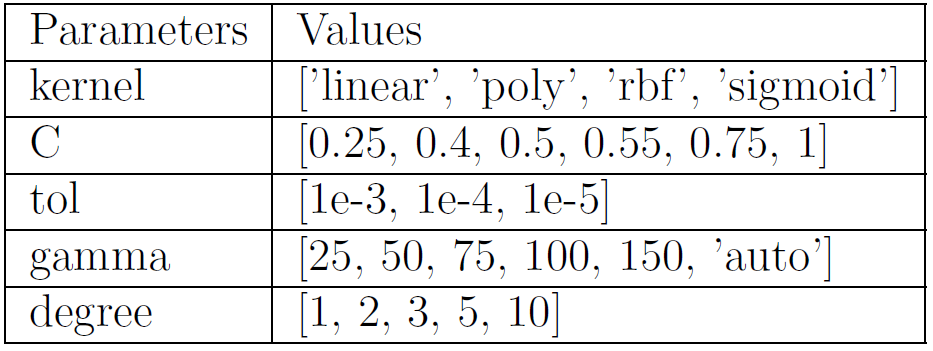
\includegraphics[width=\textwidth]{../images/results/svm.png}
	\caption{Demonstration of features transformation $x_2 = (x_1^2) $ to find non-linear relationships. Adapted from the book "Hands on Machine Learning with Scikit-Learn and TensorFlow" \cite{geron2017hands}.} 
	\label{fig:svm}
\end{figure}

So in Machine Learning, a kernel is a function capable of calculating the dot product of the transformed vectors based on the original ones. Some common kernels are Linear, Gaussian Radial Basis Function, Polynomial and Sigmoid. 

The following method described is Decision Trees. Decisions Trees, the unitary block of Extra-Trees, are a group of sequential if-then-else rules (nodes) that break down the dataset in ever so smaller subsets. These rules, are based of a single feature and threshold, which try to look for the combination that splits the data into the purest subsets. This keeps happening recursively, until it reaches the maximum depth of the tree, or until it can no longer reduce impurity. There are several criterion used to measure impurity, some of them being the Gini impurity or entropy \cite{moore2010bioinformatics,quinlan1986induction}. 

To improve on their classification power, methods which are ensembles of Decision Trees were developed. These are entire "forests" built using trees as unitary blocks, the most used being Random Forests and Extremely Randomized Trees classifiers. The Extra-Trees classifier, makes use of a set number of Decision Trees, where at each node, only a subset of random features is considered. Also, rather than searching for the best possible thresholds, it utilizes random ones too. Then, to make predictions, all the votes from every single tree are counted to output a final decision. Feature importances are calculated according to their depth in each tree. Features with high purity are usually the first ones being selected for a rule, which makes their importance score higher \cite{geurts2006extremely}. This exact process can be seen on figure \ref{fig:rf_flow}. Random Forests  work in a very similar way, but the best possible thresholds are calculated, which makes them more computationally heavier than the former, although slightly more accurate \cite{breiman2001random}. Both methods are easily interpretable and applicable in case-control studies, and are highly adaptive to data, which makes them effective when dealing with "large $p$, small $n$" problems. Besides these advantages, they also account for interaction between variables, making them tailored to detect epistasis \cite{chen2012random}. These classifiers can be used to perform \gls{SNP}s selection, genotype-phenotype association, epistasis detection and risk assessment \cite{meng2009performance, hwang2017biological}. 

\begin{figure}[h]
	\centering
	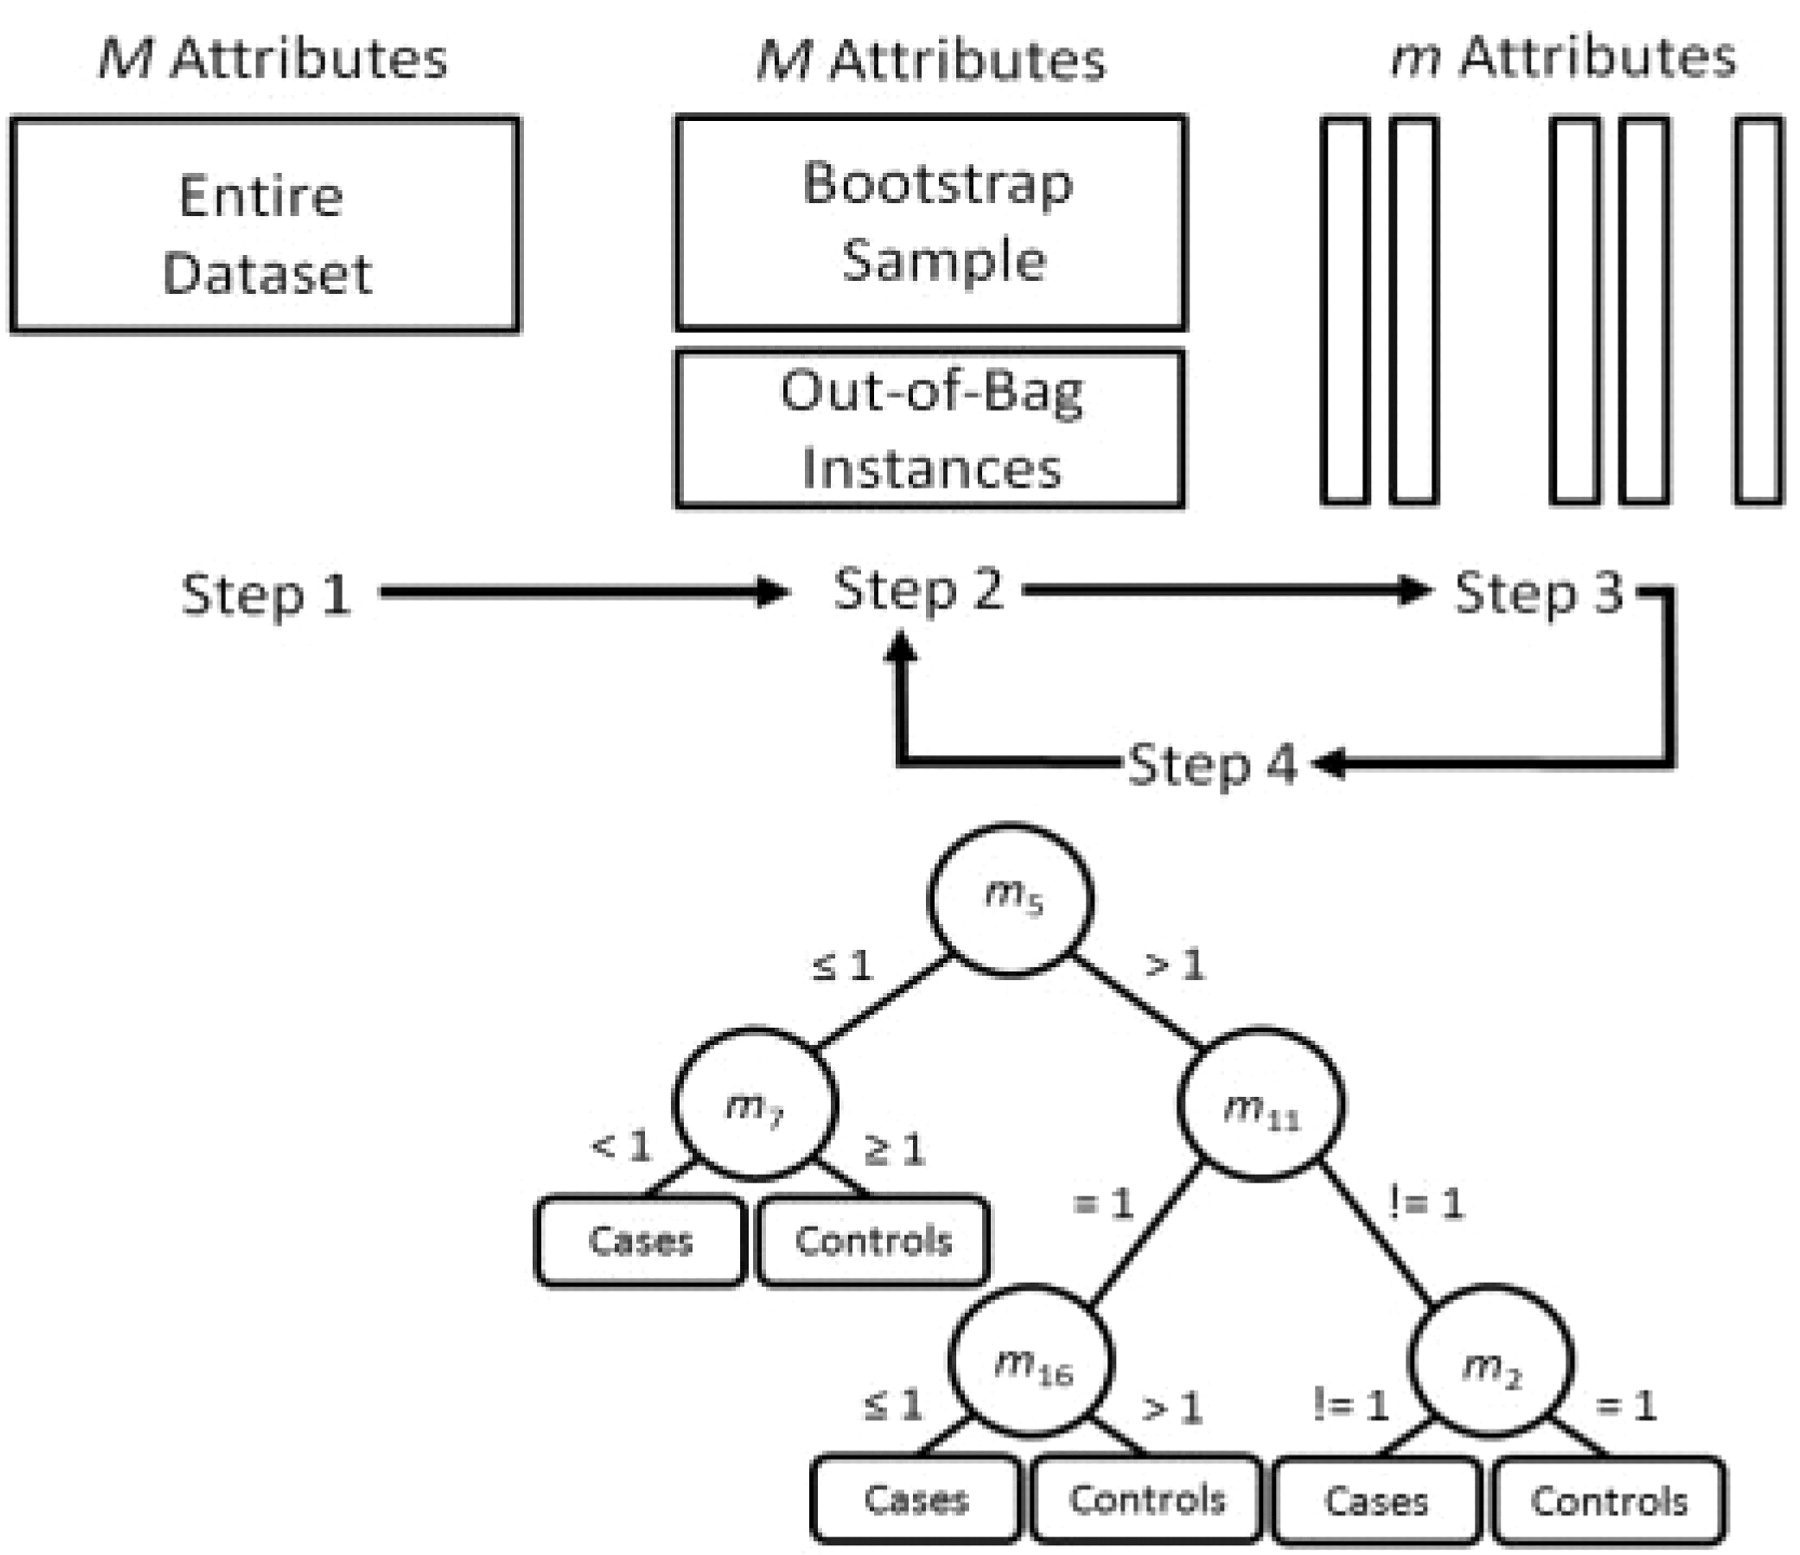
\includegraphics[width=4in]{../images/sota/btp713f1.jpeg}
	\caption{Iteration process to develop an ensemble of Decision Trees such as Random Forests or Extremely Randomized Trees classifiers. Image from "Bioinformatics challenges for genome-wide association studies" \cite{moore2010bioinformatics}.} 
	\label{fig:rf_flow}
\end{figure}

Neural Networks, more specifically, Deep Learning, is a technique based on the architecture of the biological brain, that turned out to be very good at discovering non-linear patterns in high-dimensional raw data, without much human supervision \cite{mamoshina2016applications}. The unit of a Neural Network is the neuron, which is inter-linked with other neurons in multiple layers. There is always an input layer, which feeds the hidden layers, and that ultimately leads to the output layer. Deep Learning is considered to be a Neural Network with several hidden layers (more than 3). Each neuron's output is given by the weighted sum of outputs in the layers below, to which is applied a non-linear activation function. For example, the output of the j\textsuperscript{th} neuron is given by: 
\begin{equation}
f(a\textsubscript{j}) = f(\sum_{i}^{}W\textsubscript{ij}X\textsubscript{i} + b\textsubscript{i})
\end{equation}
, where $W$ is the weight of the neuron $X$ and $b$ is bias \cite{lecun2015deep}. To perform backward propagation, the outputs are compared with the correct answer, and error derivatives are obtained. These are used to adjust the weights and improve the outputs of the network \cite{lecun2015deep, uppu2016towards}. Deep Neural Networks have produced extremely good results in the fields of image and language processing, and speech recognition. These challenges are similar in their high dimensionality and noise rates when compared to  genotype-phenotype association problems. Some studies have used such methods to detect \gls{SNP} interactions and perform \gls{GWAS} in \gls{T2D}, but they are very recent, albeit showing promising results \cite{uppu2016deep, fergus2018utilising, kim2017genetic}.

\gls{DNN}'s have many benefits, but they also come with some drawbacks. For now, they lack an adequate formulation, and are considered black boxes, which makes it hard to interpret them. When uncovering associations in \gls{GWAS} it is important to not lose track of the biological context of the problem, and that can be very hard when dealing with \gls{DNN}'s \cite{mamoshina2016applications}.

Overall, work flow of the processes used is roughly the same as shown in figure \ref{fig:flow}, and this is one of the aspects that this work aspires to change.

\begin{figure}[h]
	\centering
	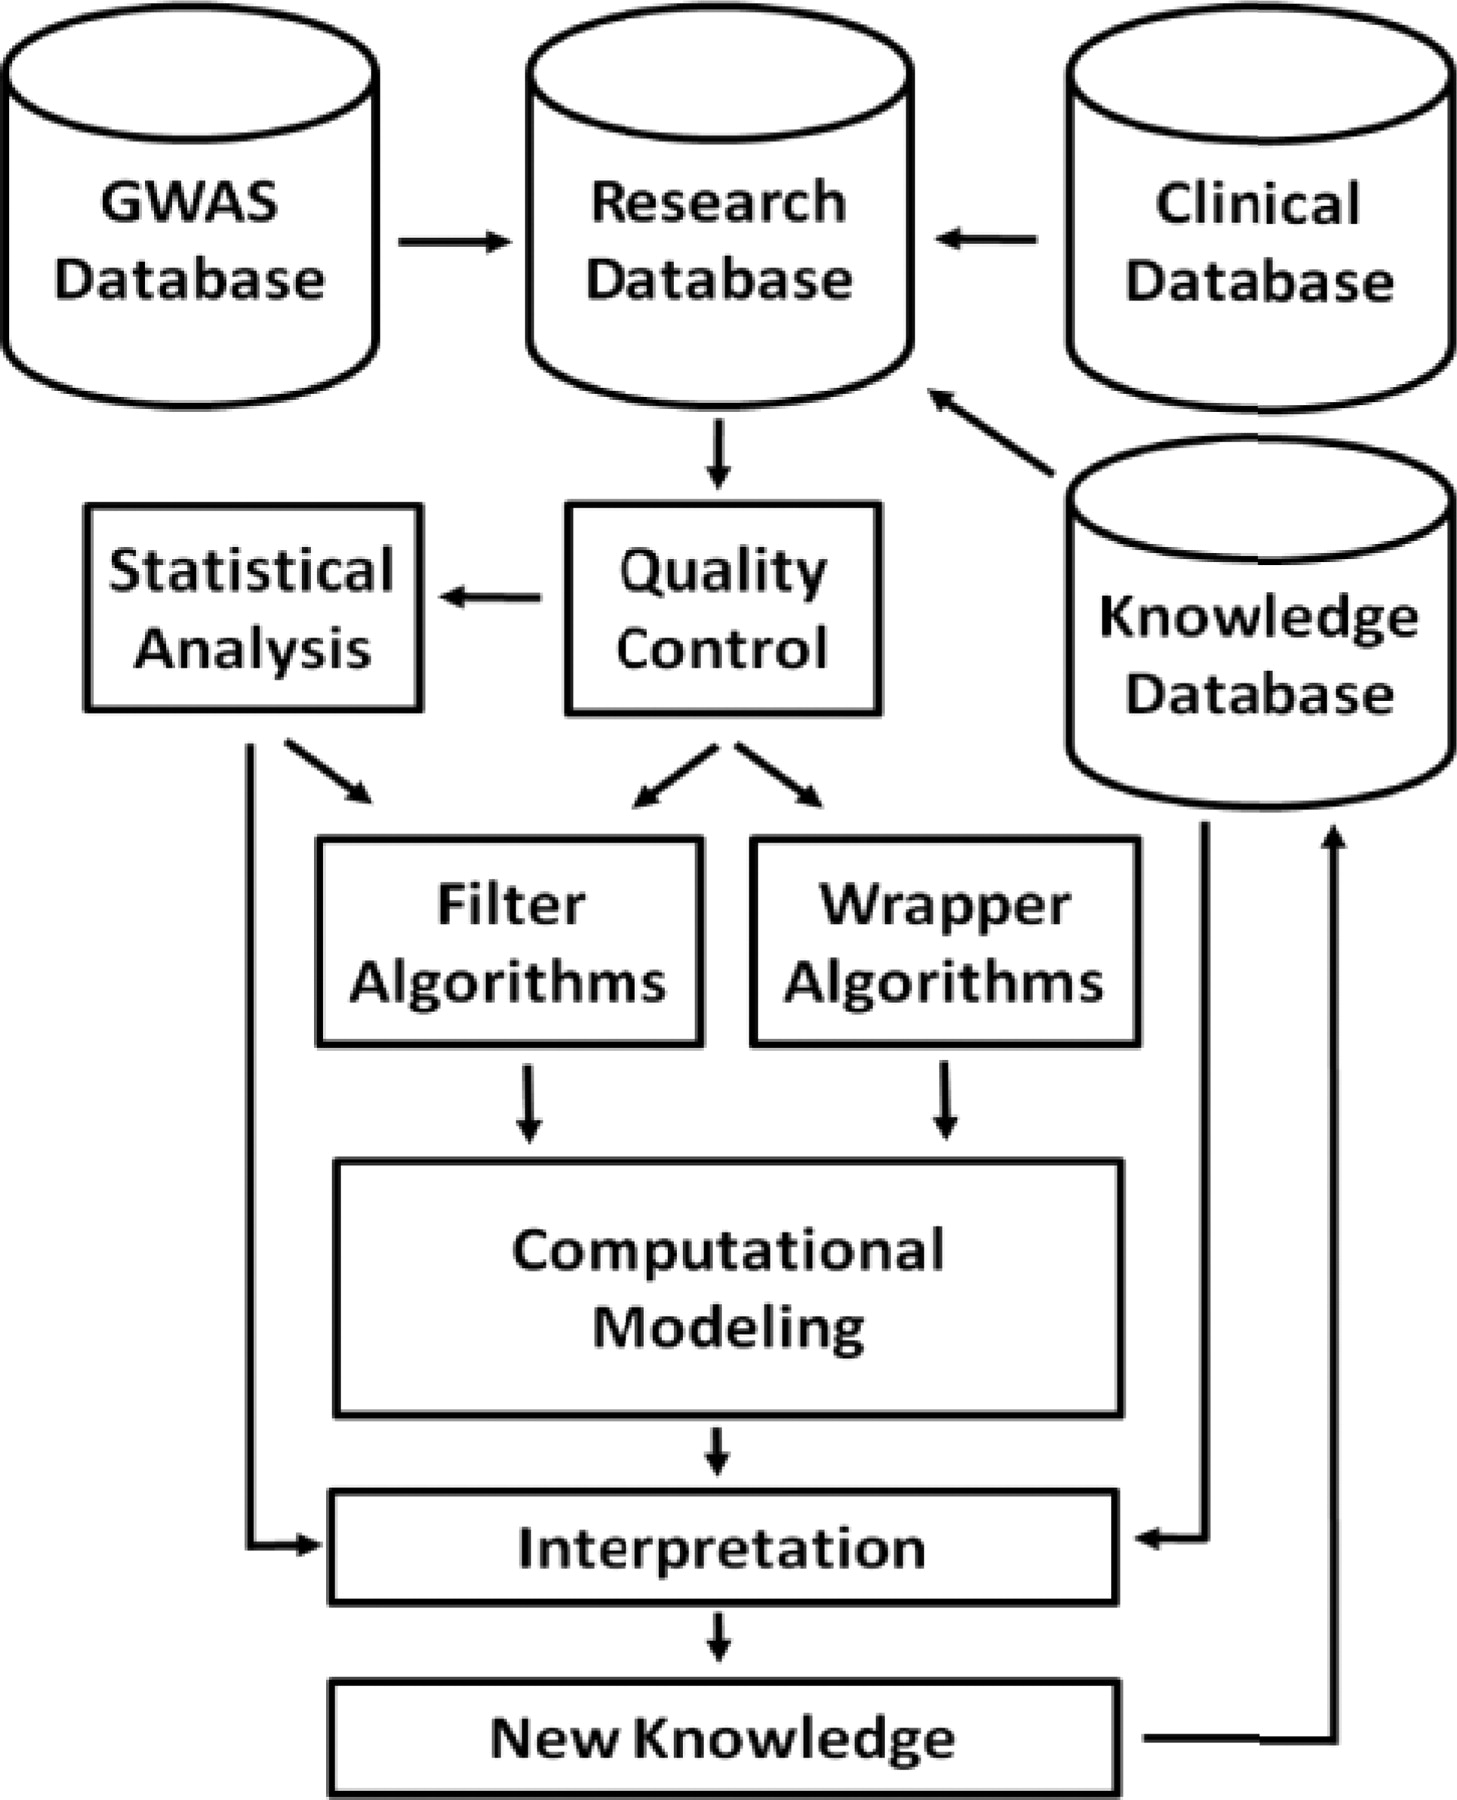
\includegraphics[width=3in]{../images/sota/btp713f5.jpeg}
	\caption{Regular work flow of projects that utilize computational methods in \gls{GWAS}. Image from "Bioinformatics challenges for genome-wide association studies" \cite{moore2010bioinformatics}.} 
	\label{fig:flow}
\end{figure}

\section{Validation of Machine Learning Methods}

Machine Learning methods bring many advantages to \gls{GWAS}, but they require proper validation so that we can be somewhat confident of their results. To perform validation, usually the available dataset is divided into a training set for the classifier to learn, and a test set, where it is analysed how it performs when introduced to new cases.

One method that is widely used to investigate overfitting is cross-validation. What this approach does is divide the dataset in $k$ folds, and use them to train and test by turns. By using it, it is possible to verify how the validation metrics come up with different combinations of training and testing. If the classifier is indeed overfitting, the metrics will fluctuate a lot more, and some runs will output very poor results \cite{Refaeilzadeh2009}. A visualization for better understanding of how this method operates can be seen on figure \ref{fig:cross_val}. 

\begin{figure}[h]
	\centering
	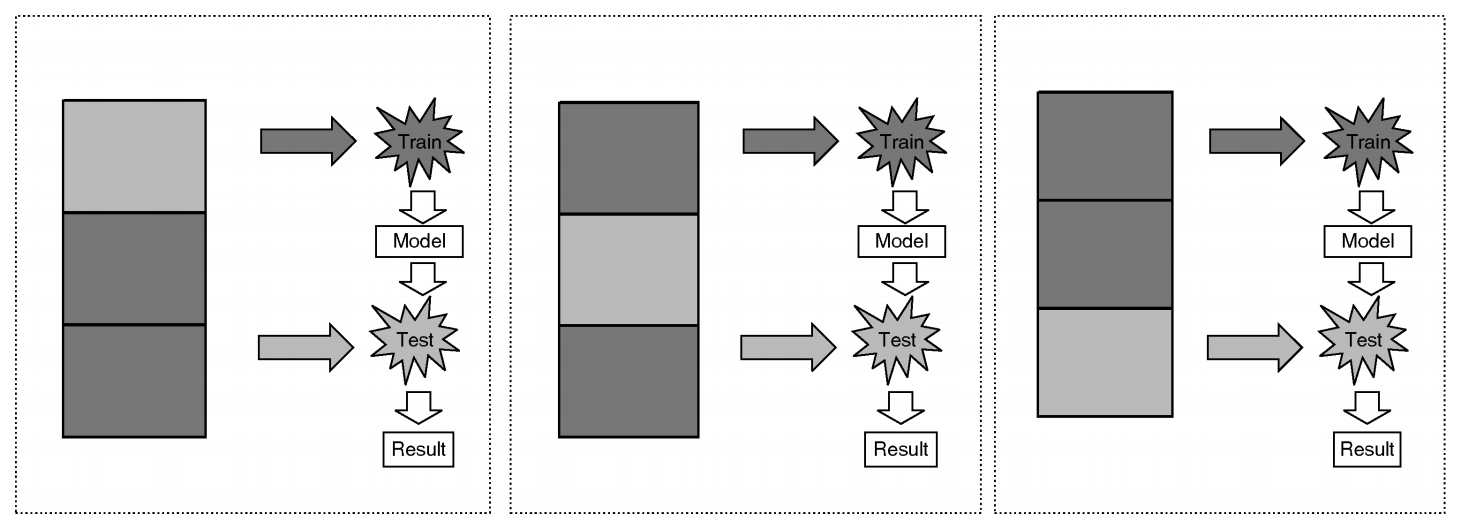
\includegraphics[width=\textwidth]{../images/results/cross_val.png}
	\caption{Demonstration of three-fold cross-validation. The same principle is applied to any k-fold cross-validation. Adapted from "Cross-Validation" \cite{Refaeilzadeh2009}.} 
	\label{fig:cross_val}
\end{figure}

There are many metrics used to draw conclusions from these tests. Intuitively, one of the first metrics to look at is the percentage of predictions that were correctly made, designated accuracy. However, in some cases, it can be misleading and display values considered good, and the classifier stills turns out to be a poor one. This can happen for example, when the dataset is greatly unbalanced, and classifies only one of the classes correctly. To avoid this, it is also important to look at sensitivity (also called True Positive Rate or Recall) and specificity (or True Negative Rate). These metrics allow to understand how well the predictions went on both classes. Another one of these metrics used is the F1-Score (or F-measure), that combines both precision and recall to output an overall goodness-of-classification metric, although it fails to consider True Negatives \cite{powers2011evaluation}. All the previously described metrics calculations can be observed in figure \ref{fig:metrics}. 

\begin{figure}[h]
	\centering
	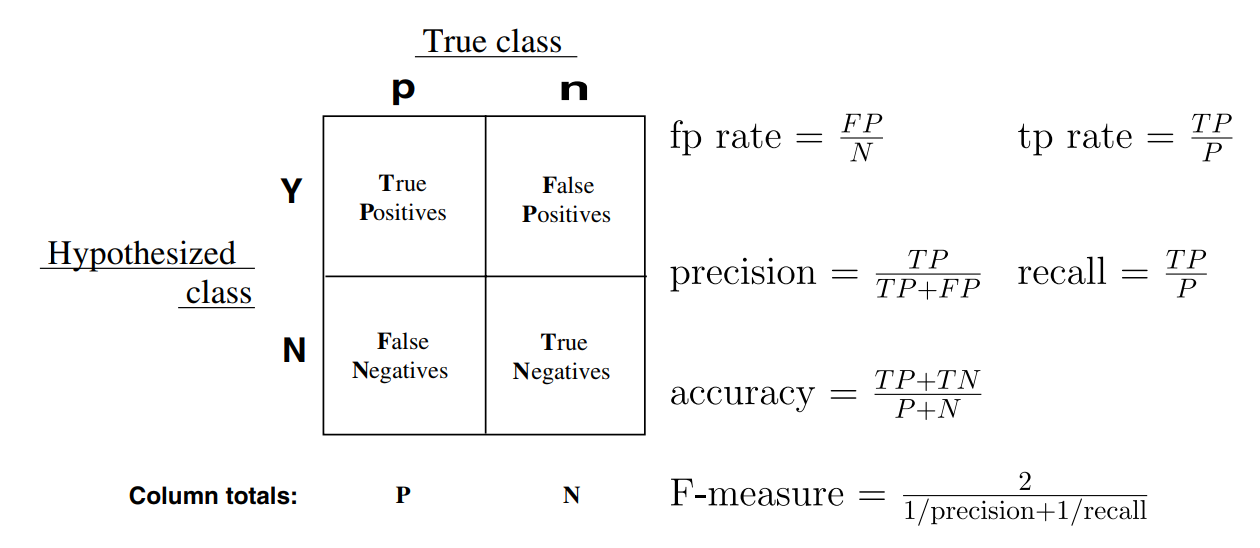
\includegraphics[width=\textwidth]{../images/results/metrics.png}
	\caption{Several Machine Learning validation metrics and how to perform their calculations. Adapted from "An Introduction to ROC analysis" \cite{fawcett2006introduction}.} 
	\label{fig:metrics}
\end{figure}

The last metric covered, that is also very widely used to analyse the best decision thresholds are the Receiver Operating Characteristics. These are meant to evaluate the discriminant power of binary classifiers at different decision thresholds. For each threshold, the corresponding True Positive rate and False Positive Rate are plotted, which serves to find the best possible trade-off between these two metrics. Lastly, the Area Under Curve (\gls{AUC}) is measured to get a picture of the global decision power for the predictor \cite{fawcett2006introduction}.